\documentclass[notitlepage, superscriptaddress]{revtex4-2}
% \documentclass[aps, prl, preprint, superscriptaddress, longbibliography]{revtex4-1}


%%%%%%%%%%%%%%%%%%%%%%%%%%%%%%%%%%%%%%%%%%%%%%%%%%%%%%%%%%%%%%%%%%%%%
\usepackage{amsmath}
\usepackage{hyperref}
\usepackage{latexsym}
\usepackage{graphicx}
\usepackage[usenames,dvipsnames]{xcolor}
\usepackage{bm}
\usepackage[normalem]{ulem}


\begin{document}

\title{SEIR-C: An epedemic model that includes contact tracing}

\author{Lynden K. Shalm}
\affiliation{National Institute of Standards and Technology, 325 Broadway, Boulder, CO 80305, USA}


% \author{Sae Woo Nam}
% \affiliation{National Institute of Standards and Technology, 325 Broadway, Boulder, CO 80305, USA}

\begin{abstract}
The SEIR model has been widely used to study the dynamics of pandemics. Here we update the model to include the effects of contact tracing as a means to control the outbreak. We call this new model SEIR-C.
\end{abstract}
\date{\today}
\maketitle

\section{Introduction}
The SEIR model relies on a set of differential equations to model the transmission dynamics of an infectious disease. A susceptible population ($S$) has some probability of coming into contact with the infected population ($I$) while they still infectious for some time ($\tau_{inf}$). Those from $S$ who have contracted the disease are then classified as having been exposed ($E$). Those who are exposed are not infectious, but rather the disease takes some time ($\tau_{inc}$) to incubate, after which point they move to the infectious population. Individuals who are in $I$ will eventually recover after a time $\tau_{inf}$. At this point they are assumed to have achieved immunity or have died. For the situation considered here, we also assume that birth rates and death rates are equal so the total population remains constant. 

In the standard SEIR model the rate of change for each of the different disease stages are given as a set of coupled differential equations:
\begin{eqnarray}
\label{E:SEIR}
\frac{dS}{dt} &=& - \beta_0 \frac{I}{N}S, \\
\frac{dE}{dt} &=& \beta_0 \frac{I}{N}S - \frac{1}{\tau_{inc}}E, \\ 
\frac{dI}{dt} &=& \frac{1}{\tau_{inc}}E - \frac{1}{\tau_{inf}}I, \\ 
\frac{dR}{dt} &=& \frac{1}{\tau_{inf}}I.
\end{eqnarray}

Here $\beta_0 = \frac{R_{0}}{\tau_{inf}}$, where $R_{0}$ is the average number of people an infectious person in $I$ will infect and is known known as the reproduction number. The rate at which the exposed population increases is therefore related to how fast an infectious person spreads the disease ($\beta_{0}$) times the fraction of the population that is infectous ($I/N$) multiplied by the number of people who are susceptible ($S$).

\section{SEIR-C}
Here we introduce a new layer to the model that incorporates contact tracing. Contact tracing is a method of epidemic control that relies on tracing who those infected were in contact with, and then having them self-isolate. This reduces the spread of the disease as it is possible to identify and isolate those who are infectious as well as those who could potentially become infectious. Contact tracing relies on a large portion of the population participating as well as testing a substatial fraction of the population. Here we model the dynamics of contact tracing where $p_{c}$ is the fraction of the population who choose to participate, $p_t$ is the probability of an individual getting tested in a time interval $dt$, the tests take some time $\tau_{t}$ to process, and it takes some time $\tau_{n}$ for someone who tests positive and chooses to participate to notify others they may have been in contact with. A certain percantage of the tests performed will result in either a false positive ($f_{pos}$) or a false negative ($f_{neg}$). A simplified model of SEIR-C is shown in figure \ref{f:SEIR-C}.

\begin{figure}
\centering
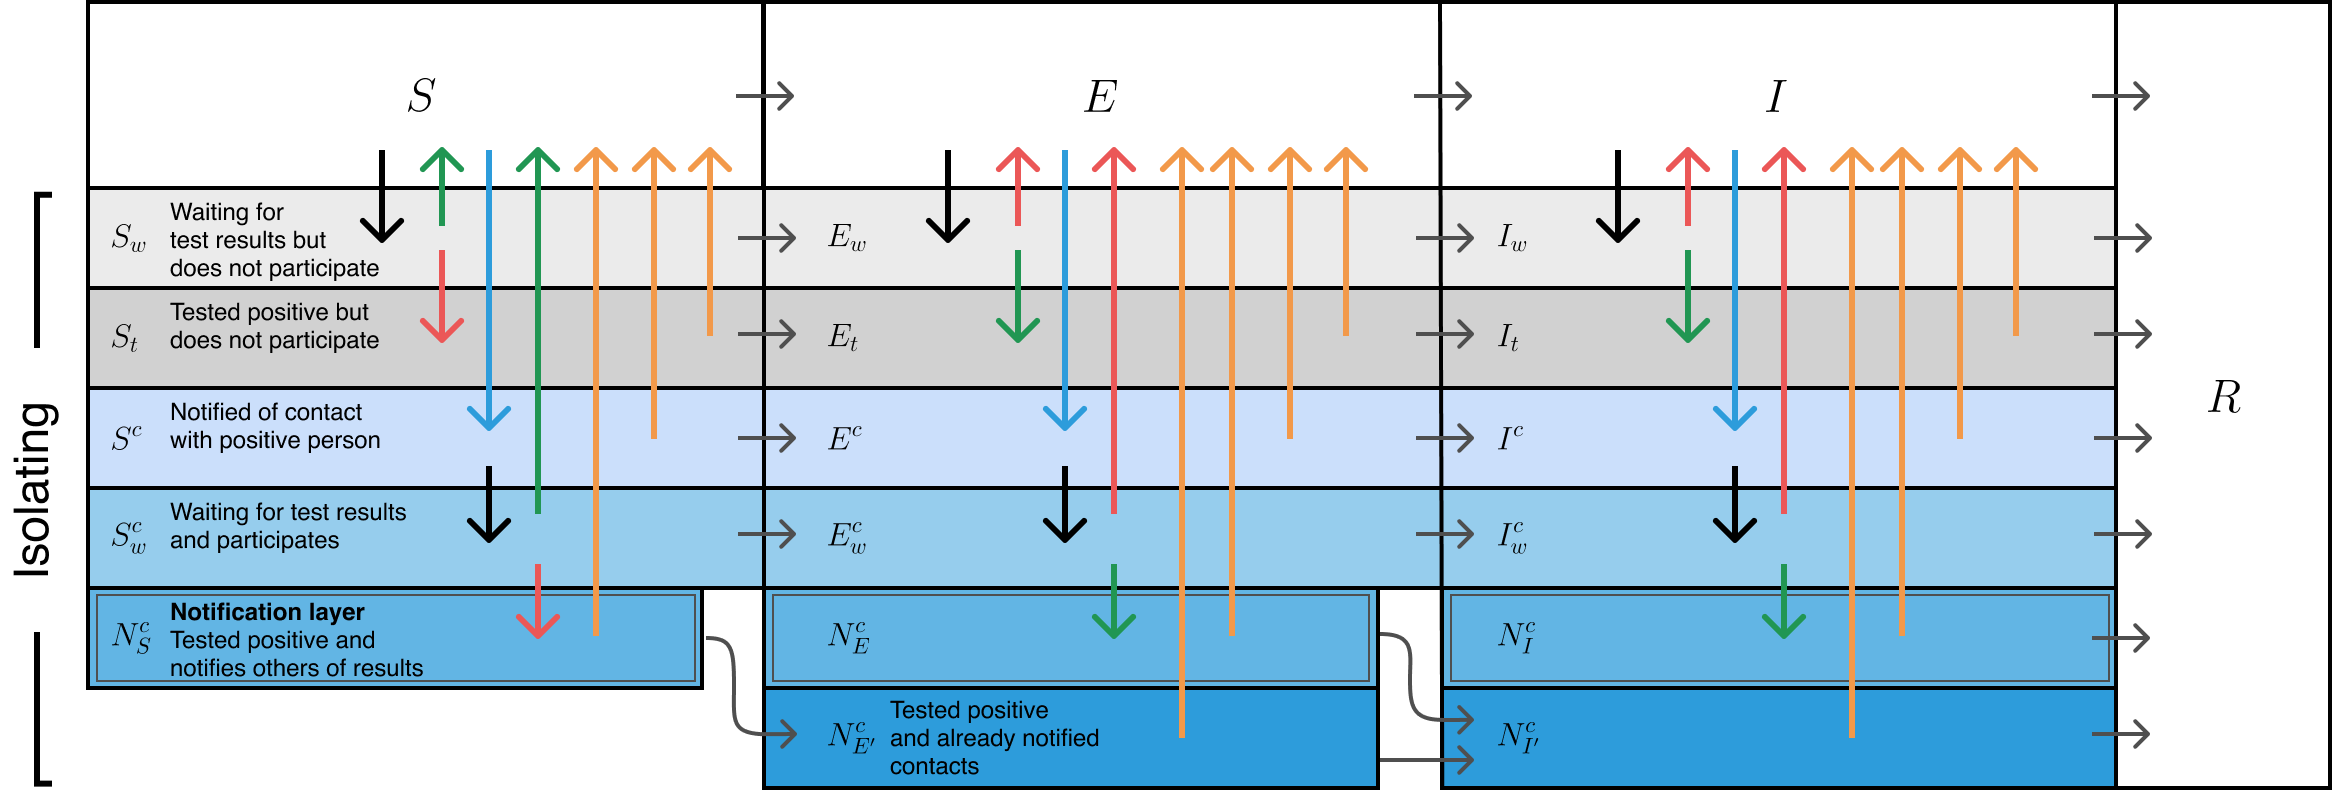
\includegraphics[width=7in]{SEIR-C_diagram.png}
\caption{\label{f:SEIR-C}
 Conceptual diagram for SEIR-C. Each of the four regions for sucesptible ($S$), exposed ($E$), infectious ($I$), and recovered $(R)$ are separated, and the red arrows represent transitions between their respective populations simialr to SEIR. However, in $S$, $E$, and $I$ there is a sub population of individuals who isolate, slowing the spread. The model assumes that during some $dt$ there is a probability of being tested $p_t$. If someone tests positive and participates in contact tracing, then they notify those that they were in contact with so those individuals can begin isolation. Anyone who tests positive or who is waiting for a test is assumed to isolate. Also, it is assumed that the isolation period is longer thant the infectious and incubation period. The black and grey arrows represent the different dynamics as individuals are moved to isolation, and the blue arrows represent notifications from those who test positive and participate in contact tracing.}
\end{figure}

To simply matters, we assume that those who are tested immediately isolate themselves while waiting for the results. We also assume that the isolation time, $\tau_{iso}$ is greater than sum of the incubation and infectious times in order to be effective. Finally, we assume that those in $S$ who self-isolate either because they are waiting for a test result or because they come in contact with an infectious individual, can't become infected until they return to the general population. Those that are infectious ($I_{iso}$), but isolating, will have a much smaller rate of passing on the infection $\beta_{iso} = \frac{R_{iso}}{\tau_{inf}}$, while those who are infectious but have not isolating ($I$) will remain infectious at a rate of $\beta_{0}$ used in the SEIR model. Anyone who has been exposed, but is now isolating either through a contact tracing notification or because they have been tested will eventually join $I_{iso}$ after an average time of $\tau_{inc}$. 

All of those who have been exposed ($E_{tot} = E + E_{iso}$) will move to the infectious stage after an average time of $\tau_{inc}$. Similarily, all those who are infectious ($I_{tot} =  I + I_{iso}$) will eventually move to $R$ after a time $\tau_{inf}$ regardless of their testing status or whether they are isolating. For each stage (except $R$), we consider six different scenarios: Those that are not self isolating ($S$, $E$, and $I$), those who have been notified of a possible exposure through contact tracing but have not yet been tested ($S^{c}$, $E^{c}$, and $I^{c}$), those who are waiting for test results but are not involved in contact tracing ($S_{w}$, $E_{w}$, and $I_{w}$), those who are waiting for test results and are involved in contact tracing ($S^{c}_{w}$, $E^{c}_{w}$, those who tested positive but are not involved in contact tracing ($S_{t}$, $E_{t}$, and $I_{t}$). The final group are those who are involved in contact tracing and have received a positive test result, and then notify others in $S$, $E$, and $I$ who might have been exposed. These are divided into two groups: those who receive a false positive test $N^{c}_{S}$ and those whose tests are correct $N^{c}_{EI}$. 

The initial set of differential equations closely follow the SEIR model, but now account for the different infectious rates between those who are isolating and those who are not. The sucesptible population, $S$, is given by:

\begin{eqnarray}
\label{E:Stot}
S_{tot} &=& S + S_{iso}, \\ 
S_{iso} &=& S^{c} + S^{c}_{w} + S_{w} + S_{t} + N^{c}_{S}
\end{eqnarray}

where $S_{tot}$ is the total susceptible population and $S_{iso}$ is the susceptible population who are isolating. Individuals from $S_{tot}$ can move to $E$ after they come in contact with an infectious individual. The rate of infection transfer for those not in isolation ($\gamma_{0}$), and those in isolation ($\gamma_{iso}$) is given as:

\begin{eqnarray}
\label{E:infectionrates}
\gamma_{0} &=& \beta_0 \frac{I}{N} \\ 
\gamma_{iso} &=& \beta_{iso} \frac{I_{iso}}{N}.
\end{eqnarray}

The rate of change of $S$ is determined by:
\begin{eqnarray}
\label{E:dS}
\frac{dS}{dt} &=& - [\gamma_{0}  + \gamma^{c} p_{c} +p_{t}] S + \frac{1}{\tau_{iso}}[S^{c} + S_{t} + N^{c}_{S}] + \frac{(1-f_{pos})}{\tau_{t}}[S_{w} + S^{c}_{w}].
% \frac{dS^{c}_{w}}{dt} &=& p_{t} (1 -p_{c}) S - [\frac{1}{\tau_{t}}  + \gamma_{iso}] S_{w}, \\
\end{eqnarray}
The first term involve populations that leave $S$ either through infection, a notification of a possible contact with an infectious person, or selection for testing. The second term represents those who have sucessfuly completed their isolation and return to $S$ or who test negative and return to $S$. Here the parameter $\gamma^{c}$ is a notification rate for those participating in contact tracing:
\begin{eqnarray}
\label{E:notificationrate}
\gamma^{c} &=& \frac{R^{c}}{\tau_{c}} \frac{N^{c}_{Tot} }{N}, \\
N^{c}_{Tot} &=& (N^{c}_{S} + N^{c}_{EI}).
\end{eqnarray}
During contact tracing, the average number of contacts that have been made by an infectious person ($N^{c}_{Tot}$) with the the recent past ($\tau_{c}$) are notified. The total population of individuals with a positive test who are participating in contact tracing is made up of those who are not infectious but received a false positive ($N^{c}_{S}$) and those who are infectious ($N^{c}_{EI}$). 

The population of $S_{iso}$ depends on five different populations. The rate of change of $S_{iso}$ therefore depends on on the rate of change of its five constituent populations. First we consider those who go into isolation because they are tested but do not participate in contact tracing. The group waits for their test results. If the results are negative, they return to $S$ but if they receive a false positive they are moved to $S_{t}$:
\begin{eqnarray}
\label{E:dS_iso}
\frac{dS_{w}}{dt} &=& p_{t} (1 -p_{c}) S - [\frac{1}{\tau_{t}}  + \gamma_{iso}] S_{w}, \\
\frac{dS_{t}}{dt} &=& \frac{f_{pos}}{\tau_{t}} S_{w} - [\frac{1}{\tau_{iso}}  + \gamma_{iso}] S_{t}\end{eqnarray}
While in $S_{w}$ or $S_{t}$ there is a chance of becoming infected and moving to the exposed stage. Since everyone that is susceptible is by definition not a carrier of the illness, any positive tests must be due to false positives. The remaing susceiptible populations are $S^{c}$, $S^{c}_{w}$, and $N^{c}_{S}$:
\begin{eqnarray}
\label{E:dSc}
 \frac{dS^{c}}{dt} &=& \gamma^{c} p_{c} S -[p_{t} +\frac{1}{\tau_{iso}} +\gamma_{iso}] S^{c}, \\
 %
 \frac{dS^{c}_{w}}{dt} &=& p_{t}p_{c} S + p_{t}S^{c} - [\frac{1}{\tau_{t}}  + \frac{1}{\tau_{iso}}  + \gamma_{iso}] S^{c}_{w}, \\ 
 %
 \frac{dN^{c}_{S}}{dt} &=& \frac{f_{pos}}{\tau_{t}} S^{c}_{w} - [\frac{1}{\tau_{iso}}  + \gamma_{iso}] N^{c}_{S}.  
\end{eqnarray}
Individuals who are notified through contact tracing to isolate are moved to $S^{c}$. Leaving $S^{c}$ occurs when an individual is slected for testing (moved to $S^{c}_{w}$), they become infected (move to $E^{c}$), or they finish isolation and return to $S$. The final sucesptible population, $N^{c}_{S}$, are those who particpate in contact tracing and receive a false positive test. This group will self isolate, and may become infectious (moving them to $E^{c}$). Once their isolation is finished they return to $S$.

The next phase in the model are those who have been exposed ($E_{tot}$). The total exposed population grows based on the number of infections caused in thos susceptible, but is reduced by those who become infectious after the incubation period, $\tau_{inc}$, is over.

\begin{eqnarray}
\label{E:Etot}
E_{tot} &=& E + E_{iso}, \\ 
E_{iso} &=& E^{c} + E^{c}_{w} + E_{w} + E_{t} + N^{c}_{E}
\end{eqnarray}

The rate of change of $E$ is determined by:
\begin{eqnarray}
\label{E:dE}
\frac{dE}{dt} &=& \gamma_{0}S  + \frac{1}{\tau_{iso}}[E^{c} + E_{t} + N^{c}_{E}] + \frac{f_{neg}}{\tau_{t}}[E_{w} + E^{c}_{w}] -  [\gamma^{c} p_{c} +p_{t} + \frac{1}{\tau_{inc}}] E
\end{eqnarray}

The next term is:
\begin{eqnarray}
\label{E:dE_w}
\frac{dE_{w}}{dt} &=& \gamma_{iso} S_{w} + p_{t} (1 - p_{c}) E - [\frac{1}{\tau_{t}}  + \frac{1}{\tau_{inc}}] E_{w}, \\
\frac{dE_{t}}{dt} &=& \gamma_{iso} S_{t} + \frac{(1- f_{neg})}{\tau_{t}} E_{w} - [\frac{1}{\tau_{iso}}  + \frac{1}{\tau_{inc}}] E_{t}\end{eqnarray}

The next term is:
\begin{eqnarray}
\label{E:dEc}
 \frac{dE^{c}}{dt} &=& \gamma_{iso} S^{c} + \gamma^{c} p_{c} E -[p_{t} +\frac{1}{\tau_{iso}} + \frac{1}{\tau_{inc}}] E^{c}, \\
 %
 \frac{dE^{c}_{w}}{dt} &=& \gamma_{iso} [S^{c}_{w} + N^{c}_{S}]+ p_{t}p_{c} E + p_{t}E^{c} - [\frac{1}{\tau_{t}}  + \frac{1}{\tau_{iso}}  + \frac{1}{\tau_{inc}}] E^{c}_{w}, \\ 
 %
 \frac{dN^{c}_{E}}{dt} &=&  \frac{(1-f_{neg})}{\tau_{t}} E^{c}_{w} - [\frac{1}{\tau_{iso}}  + \frac{1}{\tau_{inc}}] N^{c}_{E}.  
\end{eqnarray}

STARTING I phase

\begin{eqnarray}
\label{E:Itot}
I_{tot} &=& I + I_{iso}, \\ 
I_{iso} &=& I^{c} + I^{c}_{w} + I_{w} + I_{t} + N^{c}_{I} + N^{c}_{I'}
\end{eqnarray}

The rate of change of $I$ is determined by:
\begin{eqnarray}
\label{E:dI}
\frac{dI}{dt} &=& \frac{1}{\tau_{inc}}E  + \frac{1}{\tau_{iso}}[I^{c} + I_{t} + N^{c}_{I} + N^{c}_{I'}] + \frac{f_{neg}}{\tau_{t}}[I_{w} + I^{c}_{w}] -  [\gamma^{c} p_{c} +p_{t} + \frac{1}{\tau_{inf}}] I
\end{eqnarray}


The next term is:
\begin{eqnarray}
\label{E:dI_w}
\frac{dI_{w}}{dt} &=& \frac{1}{\tau_{inc}} E_{w} + p_{t} (1 - p_{c}) I - [\frac{1}{\tau_{t}}  + \frac{1}{\tau_{inf}}] I_{w}, \\
\frac{dI_{t}}{dt} &=& \frac{1}{\tau_{inc}} E_{t} + \frac{(1- f_{neg})}{\tau_{t}} I_{w} - [\frac{1}{\tau_{iso}}  + \frac{1}{\tau_{inf}}] I_{t}\end{eqnarray}

%%%%%%

The next term is:
\begin{eqnarray}
\label{E:dIc}
 \frac{dI^{c}}{dt} &=& \frac{1}{\tau_{inc}} E^{c} + \gamma^{c} p_{c} I -[p_{t} +\frac{1}{\tau_{iso}} + \frac{1}{\tau_{inf}}] I^{c}, \\
 %
 \frac{dI^{c}_{w}}{dt} &=& \frac{1}{\tau_{inc}} E^{c}_{w} + p_{t}p_{c} I + p_{t}I^{c} - [\frac{1}{\tau_{t}}  + \frac{1}{\tau_{iso}}  + \frac{1}{\tau_{inf}}] I^{c}_{w}, \\ 
 %
 \frac{dN^{c}_{I}}{dt} &=&  \frac{(1-f_{neg})}{\tau_{t}} I^{c}_{w} - [\frac{1}{\tau_{iso}}  + \frac{1}{\tau_{inf}}] N^{c}_{I}, \\
 %.
 \frac{dN^{c}_{I'}}{dt} &=&  \frac{1}{\tau_{inc}} E^{c}_{I} - \frac{1}{\tau_{inf}}N^{c}_{I'}.
\end{eqnarray}


Where the total exposed population grows based on the number of infections caused in thos susceptible, but is reduced by those who become infectious after the incubation period, $\tau_{inc}$, is over. The total infectious rate and total recovered rate are identical to that from the standard SEIR model,
\begin{eqnarray}
\label{E:dItot}
\frac{dI_{tot}}{dt} &=& \frac{1}{\tau_{inc}}E_{tot} - \frac{1}{\tau_{inf}}I_{tot}, \\
\frac{dR_{tot}}{dt} &=& \frac{1}{\tau_{inf}}I_{tot}.
\end{eqnarray}

%%%%%%%%%%%%
% The first two terms corresponds to people in E contracting the illness and moving to the exposed population. The third term corresponds to the population that is participating in contact tracing and has been notified of a possible contact. They will be isolated and be moved to $S_{iso}$. Here $\gamma^{c} = \beta_{c}\frac{N_{c}}{N}$, and $\beta_c = \frac{R_c}{\tau_n}$ where $R_c$ is the average number of people an infectious person who has tested positive and is participating in contact tracing ($N_c$) has come into contact with over a time period where notification is required ($\tau_n$). Those who who are selected for testing ($p_t$) are imediately moved to $S_{iso}$ while they await for their test results an average of $\tau_t$ before moving back to $S$. After an average time $\tau_{iso}$, those in $S_{iso}$ can return to $S$.

% The next term is:
% \begin{eqnarray}
% \label{E:dEtot}
% \frac{dE_{tot}}{dt} &= [\beta_0 \frac{I}{N} + \beta_{iso} \frac{I_{iso}}{N}] S - \frac{1}{\tau_{inc}}E_{tot}, 
% \end{eqnarray}

% Where the total exposed population grows based on the number of infections caused in thos susceptible, but is reduced by those who become infectious after the incubation period, $\tau_{inc}$, is over. The total infectious rate and total recovered rate are identical to that from the standard SEIR model,
% \begin{eqnarray}
% \label{E:dItot}
% \frac{dI_{tot}}{dt} &=& \frac{1}{\tau_{inc}}E_{tot} - \frac{1}{\tau_{inf}}I_{tot}, \\
% \frac{dR_{tot}}{dt} &=& \frac{1}{\tau_{inf}}I_{tot}.
% \end{eqnarray}

% Now we must consider the rates involving the populations that are exposed ($E$) or infected ($I$) but have not been tested or notified that they need to isolate, the populations that know they need to isolate ($S_{iso}$, $E_{iso}$, and $I_{iso}$, the populations that have been notified they need to isolatebut have not been tested ($E_{c}$ and $I_{c}$), and the population of those who test positive and participate in contact tracing and need to notify their recent contacts ($N_c$). For those who are in $S_{iso}$, we assume they can only be infected at the isolation rate $\beta_{iso}$ no matter what class of infectious person they come in contact with. We therefore have:

% \begin{eqnarray}
% \label{E:dS_iso}
% \frac{dS_{iso}}{dt} &= [\gamma^{c} p_{c}+ p_{t}] S - [\frac{1}{\tau_{iso}} + \frac{1}{\tau_t} + \beta_{iso} \frac{I_{iso}}{N}] S_{iso},
% \end{eqnarray}

% Where the population of $S_{iso}$ is increased by either people in $S$ being informed of potential exposure through contact tracing or by individuals waiting for test results. Once the isolation period or the negative test results are obtained (these are individuals who have not yet been infected, and we are assuming there are no false positives), people return to $S$. There is also the chance that someone could become infected and moves to the exposed group that is isolating, $E_{iso}$. It is important to note the the population of $E$ and $I$, those who have the disease but are not isolating, is given by:

% \begin{eqnarray}
% \label{E:Etot}
% E &=& E_{tot} - E_{iso}, \\ 
% I &=& I_{tot} - I_{iso}.
% \end{eqnarray}

% The rate of change in the expose population that is isolating is given by:
% \begin{eqnarray}
% \label{E:dE_iso}
% \frac{dE_{iso}}{dt} &= \beta_{iso} \frac{I_{iso}}{N} S_{iso} +  [\gamma^{c} p_{c} + p_{t} - \gamma^{c} p_{c} p_{t}] E - \frac{1}{\tau_{inc}} E_{iso},
% \end{eqnarray}
% here the isolating population $S_{iso}$ that become exposed continue to isolate in $E_{iso}$. Also, anyone in $E$ who is participating in contact tracing and notifyied to self isolate, or have been selected for testing are moved to $E_{iso}$. Finally, to avoid double-counting we account for those who have been notified to isolate through contact tracing and being selected for testing (the $- \gamma^{c} p_{c} p_{t}E$ term). 

% Next we have the dynamics of the population $E_{c}$ who are exposed, participate in contact tracing, and have been told to isolate due to a potential interaction with an infectious person, but have not yet been tested. These numbers are already included in $E_{iso}$, but we need to separate out this sub population to properly account for who gets notified. The changes to these rates do not directly affect $E_{tot}$, but do have an effect on $N_{c}$.

% \begin{eqnarray}
% \label{E:dE_c}
% \frac{dE_{c}}{dt} &= \beta_{iso} \frac{I_{iso}}{N} \gamma^{c} p_{c} S +  \gamma^{c} p_{c} E  - [p_{t} - \frac{1}{\tau_{inc}}]E_{c},
% \end{eqnarray}
% where those in $S_{iso}$ due to being notified of possible exposure through contact tracing ($\gamma^{c} p_{c} S$) and then subsequently infected while isolating ($\beta_{iso} \frac{I_{iso}}{N}$) are moved to $E_{c}$. Additionally, anyone in $E$ who is notified of potential exposure is moved to $E_c$, but anyone in $E_c$ who is chosen for testing is removed while they wait their eventual positive result (at which point they are moved to $N_c$).

% The infectious phase follows a similar set of dynamics as the exposure phase. The rate of change in the $I_{iso}$ population is:
% \begin{eqnarray}
% \label{E:dI_iso}
% \frac{dI_{iso}}{dt} &= \frac{1}{\tau_{inc}} E_{iso} +  [\gamma^{c} p_{c} + p_{t} - \gamma^{c} p_{c} p_{t}] I - \frac{1}{\tau_{inf}} I_{iso},
% \end{eqnarray}
% where those who start in $E_{iso}$ are moved to $I_{iso}$ as we are assuming $\tau_{iso}$ is longer than the incubation of infectious phases of the illness. Similar to the dynamics of $\frac{dE_{iso}}{dt}$, population can move from $I$ through either contact notification or testing. Again we add a term to prevent double counting. We also need to account for the dynamics of the population $I_c$ who are infectious and have been notified to isolate, but have not yet been tested. This does not affect directly $I_{tot}$, but is needed for $N_{c}$. The rate of change of $I_c$ depends on the population of those originally in $E_c$ that become infectious, as well as those in $I$ who are notified to isolate. Anyone in $I_{c}$ selected for testing is removed as they wait for their eventual positive test results and subsequent inclusion into $N_c$:

% \begin{eqnarray}
% \label{E:dI_c}
% \frac{dI_{c}}{dt} &= \frac{1}{\tau_{inc}} E_{c} +  \gamma^{c} p_{c} I  - [p_{t} - \frac{1}{\tau_{inf}}]I_{c}.
% \end{eqnarray}

% Finally, the dynamics of the $N_c$ notification group that test positive and are part of contact tracing is described by:
% \begin{eqnarray}
% \label{E:dN_c}
% \frac{dN_{c}}{dt} &= \frac{p_{t}}{\tau_{t}}[p_{c}E + E_{c} + p_{c}I + I_{c}].
% \end{eqnarray}

% \bibliography{}


\end{document}


